%\section{Abstract}
%hypertension paper~\cite{DBLP:journals/esl/PandaAPR24}.
%\\


\section{Introduction}

Cardiovascular diseases (CVDs), such as stroke, hypertensive and rheumatic heart disease, and atrial fibrillation, account for nearly one-third of global deaths~\cite{who2024ncdportal}. This underscores the need for continuous cardiac monitoring to detect early warning signs of abnormalities. 

\ignore{\begin{wrapfigure}{r}{0.5\textwidth}
	%\begin{center}
	\centering
		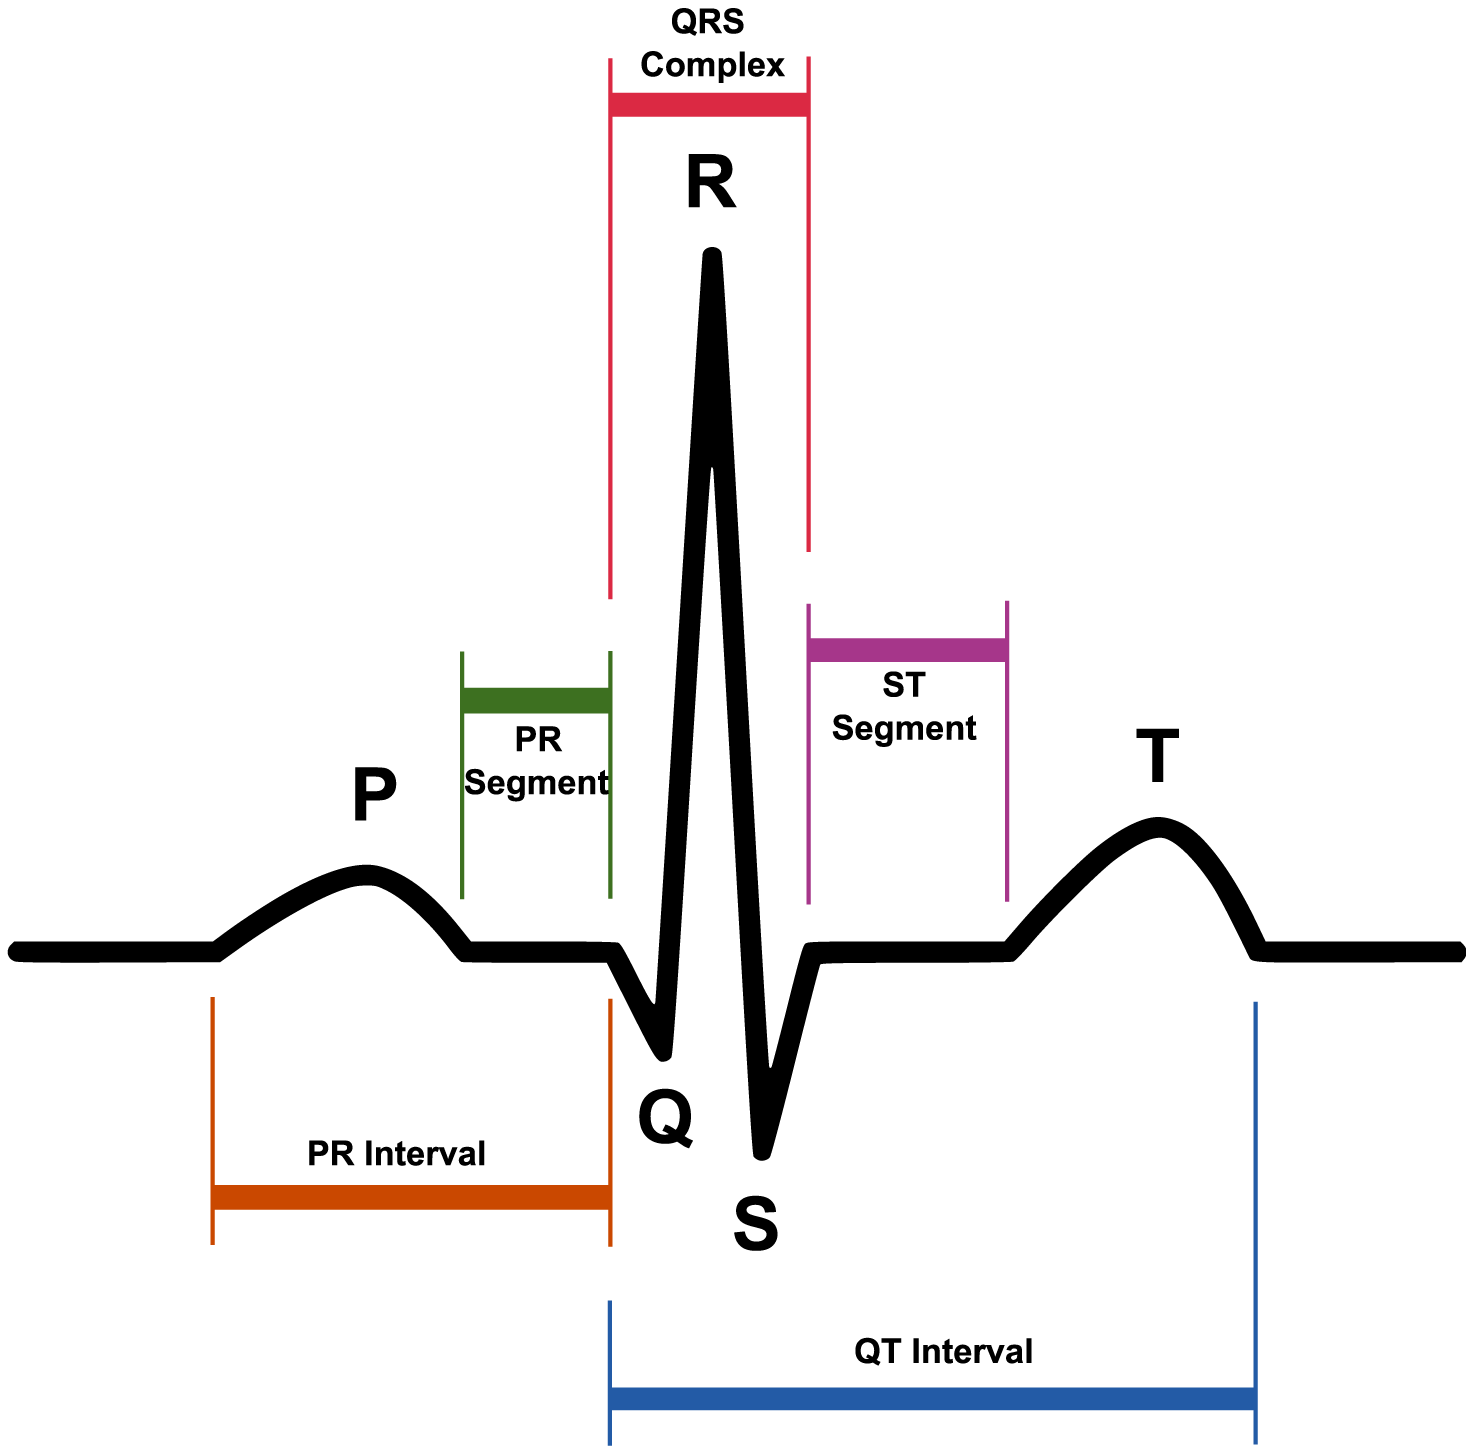
\includegraphics[width=0.2\textwidth, keepaspectratio]{Images/ECG Signal.png}
	%\end{center}
	\caption{Birds}
\end{wrapfigure}}

Electrocardiography (ECG) is the primary diagnostic tool for assessing the pathological status of the cardiac system. An ECG is a periodic signal that records electrical activity in cardiac cycle. In this context, various machine learning (ML) methods have been used for classifying ECG and detecting cardiac abnormalities~\cite{rai2013ecg,masetic2016congestive,lee2013atrial,saini2013qrs,seera2015classification}. Some research groups have attempted to detect arrhythmia in ECG data using deep learning models~\cite{malhotra2015long,chauhan2015anomaly,al2016deep}. In another study~\cite{sahoo2017multiresolution}, Sahoo~\etal propose an enhanced feature extraction (from an ECG signal) using multi-resolution wavelet transform, which helps in identifying cardiac abnormalities.

%Machine learning models have shown promising results in detecting cardiac abnormalities using ECG signals, nonetheless they do not provide any reasoning for abnormal (or normal) cardiac activity, as their internal processes are unknown. This raises the need for developing dependable and explainable techniques of health monitoring~\cite{reyes2020interpretability,gastounioti2020time}. 

\textit{Motivation:} The literature suggests that the existing studies have focused primarily on detecting the irregularity of ECG in arrhythmia. A few studies focus on periodic abnormalities in ECG that is typically observed in severe heart diseases. According to a study,
common ECG findings, that had been deemed insignificant, could indicate a risk of atrial fibrillation leading to premature death~\cite{TheHarvardGazette}. Classification of cardiac abnormalities and ECG signals using ML/deep-learning models is admirably accurate; however these models are \emph{``black-boxes''}\footnote{A \textit{``black-box''} process is one whose internal workings are unknown.}. Real-time applications of a monitor requires explainable classification of ECG signals, which would allow healthcare professionals to further assess the signal features and their implication. This raises the need for developing dependable and explainable techniques of health monitoring~\cite{reyes2020interpretability,gastounioti2020time}.

%\looseness=-2
Runtime verification (RV) is a formal verification method that monitors if a given set of system policies are satisfied during system execution. In this approach, an RV monitor is automatically synthesized from a set of formal specifications of system policies, and it can monitor these policies both online and offline. RV monitors are light-weight, and correct-by-construction; they can be easily embedded with wearable devices like smartwatches, fitness bands~\etc.

Recently, runtime verification monitors (RV) have proved to be dependable and explainable tools for online health monitoring applications like diabetes detection~\cite{panda2022policy}, safe insulin infusion system~\cite{panda2021secure}, securing pacemaker~\cite{panda2021runtime}, verifying ECG-PPG\footnote{PPG is acronym for Photoplethysmograph which is used to measure changes in blood volume.} correlation~\cite{panda2022policy}, and detecting hypertension~\cite{DBLP:journals/esl/PandaAPR24}.%~\cite{panda2021runtime,panda2021secure,panda2022novel,panda2022policy,DBLP:journals/esl/PandaAPR24}.


% in an ECG signal.
%It records the heart’s electrical activity in repeating waveforms (P-wave, QRS complex, T-wave) and remains central to diagnosis. Various machine-learning techniques, including ANNs, SVMs, random forests, KNNs, Bayesian networks, wavelet-based QRS detectors, and deep-learning arrhythmia models, have been applied to ECG classification. Yet most focus on arrhythmic irregularities, overlooking the periodic abnormalities linked to severe heart disease. Subtle ECG changes once deemed insignificant can predict future atrial fibrillation, pacemaker needs, and higher mortality. Although deep models achieve high accuracy, their “black-box” nature limits clinical trust. In response, formal runtime verification offers a dynamic, rule-based framework that both detects ECG anomalies and provides transparent, explainable results, essential for high-risk healthcare applications.


\begin{figure}
	\centering
	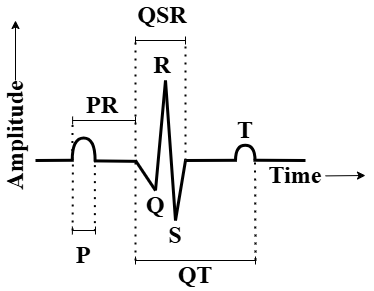
\includegraphics[scale=0.5, keepaspectratio]{Images/ECG_Final_1.png} 
	\caption{\red{A typical ECG cycle}}
\end{figure}